%%%%%%%%%%%%%%%%%%%%%%%%%%%%%%%%%%%%%%%%%
% pdflatex report.tex
%%%%%%%%%%%%%%%%%%%%%%%%%%%%%%%%%%%%%%%%%

%----------------------------------------------------------------------------------------
%	PACKAGES AND OTHER DOCUMENT CONFIGURATIONS
%----------------------------------------------------------------------------------------

\documentclass[12pt]{article}

\usepackage{fancyhdr} % Required for custom headers
\usepackage{lastpage} % Required to determine the last page for the footer
\usepackage{extramarks} % Required for headers and footers
\usepackage[usenames,dvipsnames]{color} % Required for custom colors
\usepackage{graphicx} % Required to insert images
\usepackage{listings} % Required for insertion of code
%\usepackage{courier} % Required for the courier font
%\usepackage{lipsum} % Used for inserting dummy 'Lorem ipsum' text into the template
\usepackage[utf8]{inputenc}
\usepackage[english]{babel}
\usepackage{indentfirst}
%\usepackage{url}
%\usepackage{breakurl}
\usepackage{amsmath}
\usepackage{float}

% Margins
\topmargin=-0.45in
\evensidemargin=0in
\oddsidemargin=0in
\textwidth=6.5in
\textheight=9.0in
\headsep=0.25in

\linespread{1.2}
\setlength{\parindent}{3em}
\setlength{\parskip}{1em}
\renewcommand{\baselinestretch}{1.2}

% Set up the header and footer
\pagestyle{fancy}
\fancyhead[L]{} % Top left header
\fancyhead[C]{\hmwkAuthorName} % Top center header
\fancyhead[R]{} % Top right head
\fancyfoot[L]{\hmwkTitle} % Bottom left footer
\fancyfoot[C]{} % Bottom center footer
\fancyfoot[R]{Page \thepage\ of \protect\pageref{LastPage}} % Bottom right footer
\renewcommand\headrulewidth{0.4pt} % Size of the header rule
\renewcommand\footrulewidth{0.4pt} % Size of the footer rule

%\setlength\parindent{0pt} % Removes all indentation from paragraphs

\makeatletter
\renewcommand\@biblabel[1]{}
\makeatother

\newcommand{\urlformat}[1]{\underline{#1}}

%----------------------------------------------------------------------------------------
%	CODE INCLUSION CONFIGURATION
%----------------------------------------------------------------------------------------

\definecolor{pblue}{rgb}{0.13,0.13,1}
\definecolor{pgreen}{rgb}{0,0.5,0}
\definecolor{pred}{rgb}{0.9,0,0}
\definecolor{pgrey}{rgb}{0.46,0.45,0.48}

\definecolor{MyDarkGreen}{rgb}{0.0,0.4,0.0} % This is the color used for comments
\lstloadlanguages{Python}
\lstset{language=Python,
	showspaces=false,
	showtabs=false,
	breaklines=true,
	showstringspaces=false,
	breakatwhitespace=true,
	commentstyle=\color{pgreen},
	keywordstyle=\color{pblue},
	stringstyle=\color{pred},
	basicstyle=\small,
	moredelim=[il][\textcolor{pgrey}]{$$},
	moredelim=[is][\textcolor{pgrey}]{\%\%}{\%\%}
}

%----------------------------------------------------------------------------------------
%	NAME AND CLASS SECTION
%----------------------------------------------------------------------------------------

\newcommand{\hmwkTitle}{CO528 Intelligent systems Assessment: Genetic Algorithms}
\newcommand{\hmwkDueDate}{March 7, 2016}
\newcommand{\hmwkAuthorName}{Colin Julien, Maigret Aurelien, Roy Antoine, Zajda Florent}

%----------------------------------------------------------------------------------------
%	TITLE PAGE
%----------------------------------------------------------------------------------------

\title{
\vspace{2in}
\Huge{\textmd{\textbf{\hmwkTitle}}}
\vspace{3in}
}

\author{
	\textbf{Colin Julien (jrfc2)}
	\and
	\textbf{Maigret Aurelien (am2074)}
	\and
	\textbf{Roy Antoine (ar502)}
	\and
	\textbf{Zajda Florent (fz41)}
}
\date{\hmwkDueDate}

%----------------------------------------------------------------------------------------

\begin{document}

\maketitle

%----------------------------------------------------------------------------------------
%	TABLE OF CONTENTS
%----------------------------------------------------------------------------------------

%\setcounter{tocdepth}{1}
%\newpage
%\tableofcontents
%\newpage

%----------------------------------------------------------------------------------------
%	SECTIONS
%----------------------------------------------------------------------------------------

\newpage

% --------------------- Example

%\section{Title}

%\begin{lstlisting}[frame=single,caption=Source code title]
%CODE
%\end{lstlisting}

%\lipsum[3]

% --------------------- Content

\section{Source code}

\begin{lstlisting}[frame=single,caption=Compute of the fitness value]
import random
import math
import plotly

# Polynomial Function settings
DATA_FILENAME    = "data.in"
SIZE_COEFFICIENT = 6
MIN_COEFFICIENT  = -1000.0
MAX_COEFFICIENT  = 1000.0

# Genetic Algorithm settings
POP_SIZE         = 500
NUMBER_OF_TURNS  = 2000
PROBA_CROSSOVER  = 0.90
PROBA_MUTATION   = 0.01
RATE_MUTATION    = 0.00001


# Fetching data
target_x = list()
target_y = list()

with open(DATA_FILENAME) as input_file:
    for line in input_file:
        numbers = line.strip().split()
        if len(numbers) == 2:
            target_x.append(float(numbers[0]))
            target_y.append(float(numbers[1]))


# Compute value from a X and a coefficients list
def compute_value(coefs, x):
    # In order to have faster computations, we preferred not to use our original function (which is 3 times slower).
    # -------------------
    # value = 0
    # for coef in range(SIZE_COEFFICIENT):
    #     value += coefs[coef] * x**coef
    # return value
    return coefs[0] + coefs[1] * x + coefs[2] * x**2 + coefs[3] * x**3 + coefs[4] * x**4 + coefs[5] * x**5


# Class for each Individual Solution
class IndividualSolution:
    def __init__(self, coefs):
        self.coefs = coefs
        self.fitness = 0
        for index in range(len(target_x)):
            self.fitness += abs(target_y[index] - compute_value(self.coefs, target_x[index]))

    def mutation(self):
        index = random.randint(0, SIZE_COEFFICIENT - 1)
        mutation_value = abs(RATE_MUTATION * self.coefs[index])
        if random.random() < 0.5:
            mutation_value *= -1
        self.coefs[index] += mutation_value

    def crossover(self, other): # linear crossover - Wright 1991
        coefs1, coefs2, coefs3 = [], [], []
        for index in range(SIZE_COEFFICIENT):
            coefs1.append(0.5 * self.coefs[index] + 0.5 * other.coefs[index])
            coefs2.append(1.5 * self.coefs[index] - 0.5 * other.coefs[index])
            coefs3.append(-0.5 * self.coefs[index] + 1.5 * other.coefs[index])
        childs = [IndividualSolution(coefs1), IndividualSolution(coefs2), IndividualSolution(coefs3)]
        return sorted(childs, key=lambda x: x.fitness)[:2]


# Breeding (Crossover + Mutation on 2 individuals)
def breeding(ind1, ind2):
    if random.random() < PROBA_CROSSOVER:
        ind1, ind2 = ind1.crossover(ind2)
    if random.random() < PROBA_MUTATION:
        ind1.mutation()
    if random.random() < PROBA_MUTATION:
        ind2.mutation()
    return ind1, ind2


# Generate the next population
def next_pop(pop):
    pop = sorted(pop, key=lambda x: x.fitness)
    new_pop = list()
    new_pop.append(pop[0])
    for i in range(math.floor(POP_SIZE / 2)):
        new_pop.extend(breeding(pop[i * 2], pop[i * 2 + 1]))
    return new_pop[:POP_SIZE]


# Generate a random solution
def random_solution():
    solution = list()
    for _ in range(SIZE_COEFFICIENT):
        solution.append(random.uniform(MIN_COEFFICIENT, MAX_COEFFICIENT))
    return solution


# Generate an initial random population
pop = [IndividualSolution(random_solution()) for _ in range(POP_SIZE)]
fitness = []

for turn in range(NUMBER_OF_TURNS):
    # Generate the next population
    pop = next_pop(pop)

    # Compute the fitness evolution
    fitness.append([pop[0].fitness, pop[-1].fitness, sum(x.fitness for x in pop) / POP_SIZE])

    # ------------- DEBUG MESSAGE -------------
    if turn % (math.floor(NUMBER_OF_TURNS / 100)) == 0:
        print("%3d%%: %s  Fitness:%f" % (math.floor(turn / NUMBER_OF_TURNS * 100), str(pop[0].coefs), pop[0].fitness))
    # -----------------------------------------


# Selection of the best solution
best = pop[0]
print("\nBest solution: %s  Fitness: %f" % (best.coefs, best.fitness))


# Generation of the graphs

generated_x = list()
generated_y = list()
for index in range(len(target_x)):
    generated_x.append(target_x[index])
    generated_y.append(compute_value(best.coefs, target_x[index]))

plotly.offline.plot({
        "data": [
            plotly.graph_objs.Scatter(x=target_x, y=target_y, name='Target curve'),
            plotly.graph_objs.Scatter(x=generated_x, y=generated_y, name='Generated curve')
        ],
        "layout": {
            "title": "Reproduce a curve using a Genetic Algorithm",
            "xaxis": { "title": "x" },
            "yaxis": { "title": "y" }
        }
    },
    filename='compare-results.html')

plotly.offline.plot({
        "data": [
            plotly.graph_objs.Scatter(x=list(range(len(fitness))), y=list(map(lambda x: x[0], fitness)), name='Minimun fitness'),
            plotly.graph_objs.Scatter(x=list(range(len(fitness))), y=list(map(lambda x: x[1], fitness)), name='Maximum fitness'),
            plotly.graph_objs.Scatter(x=list(range(len(fitness))), y=list(map(lambda x: x[2], fitness)), name='Average fitness'),
        ],
        "layout": {
            "title": "Evolution of fitness during a Genetic Algorithm",
            "xaxis": { "title": "iteration" },
            "yaxis": { "title": "fitness value" }
        }
    },
    filename='compare-fitness.html')
\end{lstlisting}

\section{Plot of the target curve}

\begin{figure}[H]
	\centering
	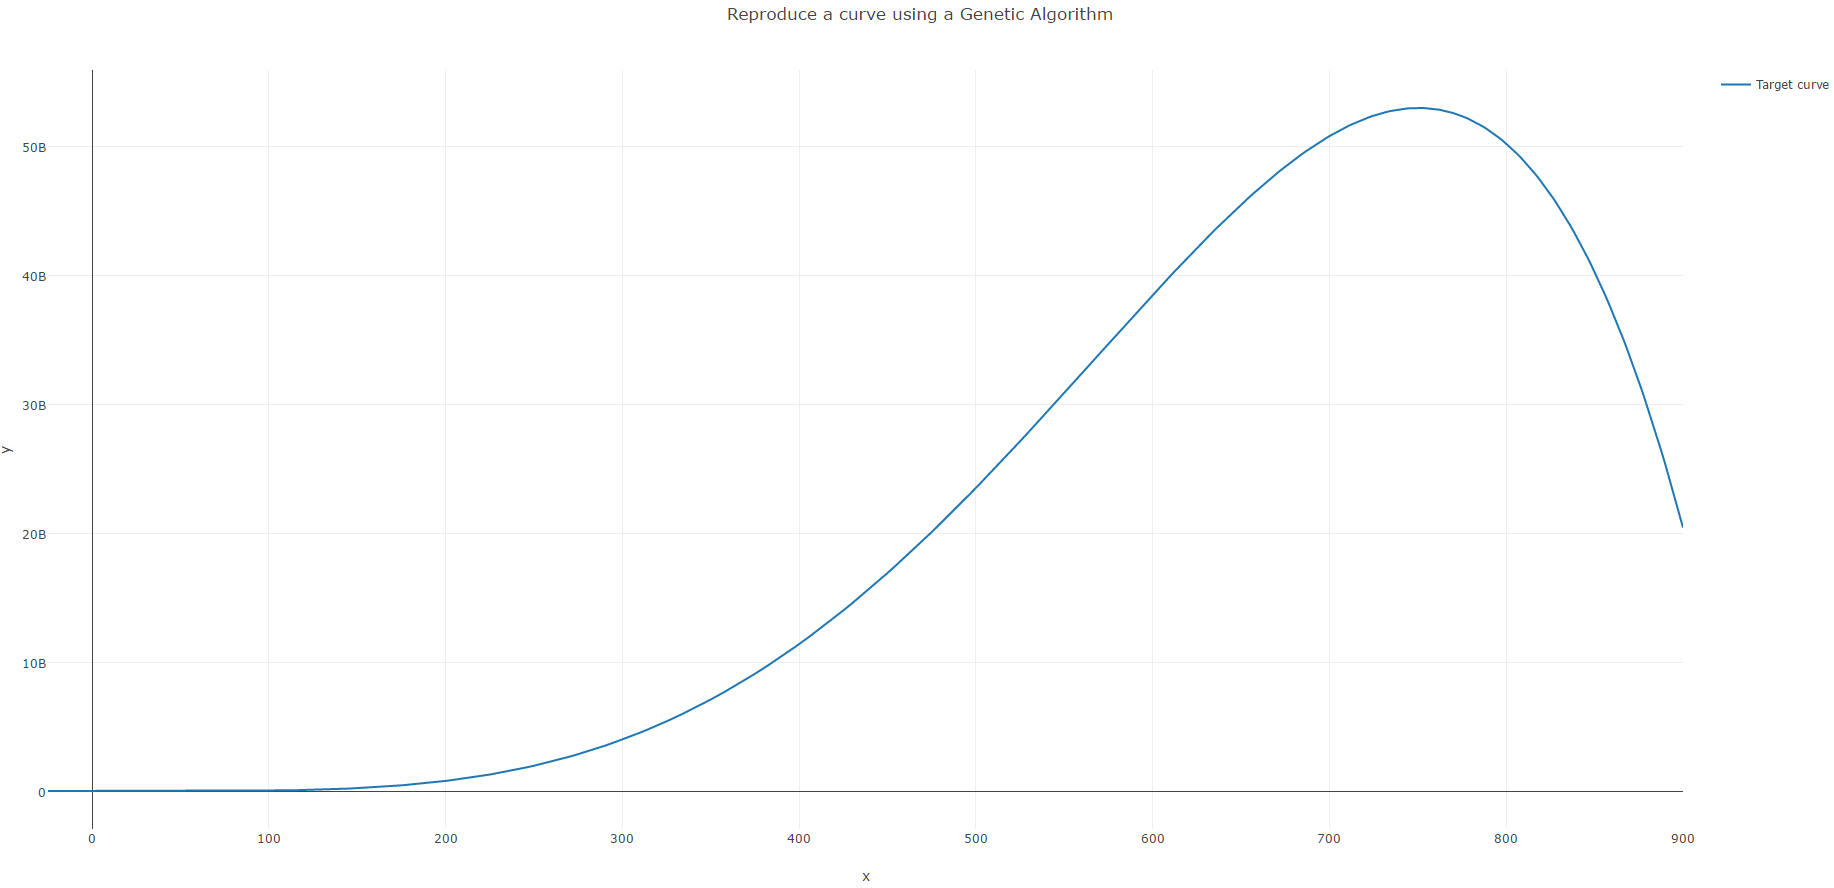
\includegraphics[width=1.0\columnwidth, angle=270]{./plot_target.png}
	\caption{Target curve}
\end{figure}

\section{Description of our Genetic Algorithm}

We randomly generate a population of 500 solutions. Each solution consists of 6 numbers between -1000 and 1000 representing the a,b,c,d,e,f coefficients of the given polynomial function. We determine the fitness of every solution by using these coefficients for the polynomial function and comparing the results to the points given in the data file that we use as input. We then store the absolute value of the fitness for later use.

The next step is modifying the population. To do that, we order the solutions of the current population by their fitness in an ascending order, 0 being the best solution.

We keep the first solution, the one that has the best fitness and we do not modify it. We then cycle through all the population, working with 2 solutions at a time.

With these 2 solutions we are going to generate 3 offsprings. Firstly, we generate a random number between 0 and 1 corresponding to the probability that crossover will be applied to that pair. Secondly, we use Wright's linear crossover method to create 3 offsprings (with parents a and b, this method gives us 3 results consisting of $0.5a + 0.5b$, $1.5a – 0.5b$ and $-0.5a + 1.5b$). Of these 3 offsprings, we select the 2 with the best fitness and use them for our new population instead of their parents. But before that, thirdly, there is a probability that a slight mutation will be applied to them. We chose a probability of 0.9 for the use of crossover and 0.01 for the mutation, with a mutation rate of 0.00001 since we realised that the most important part of the algorithm here was the crossover. We took in account the fact that a solution could be so good that it did not need any crossover or mutation, even if it is very unlikely, hence the values we used for the probabilities.

We then have our new population, which is going to undergo the same steps, and so for a total of 1500 times and give us a solution with a fitness close to 0.

\section{Plot of the Fitness variation}

\begin{figure}[H]
	\centering
	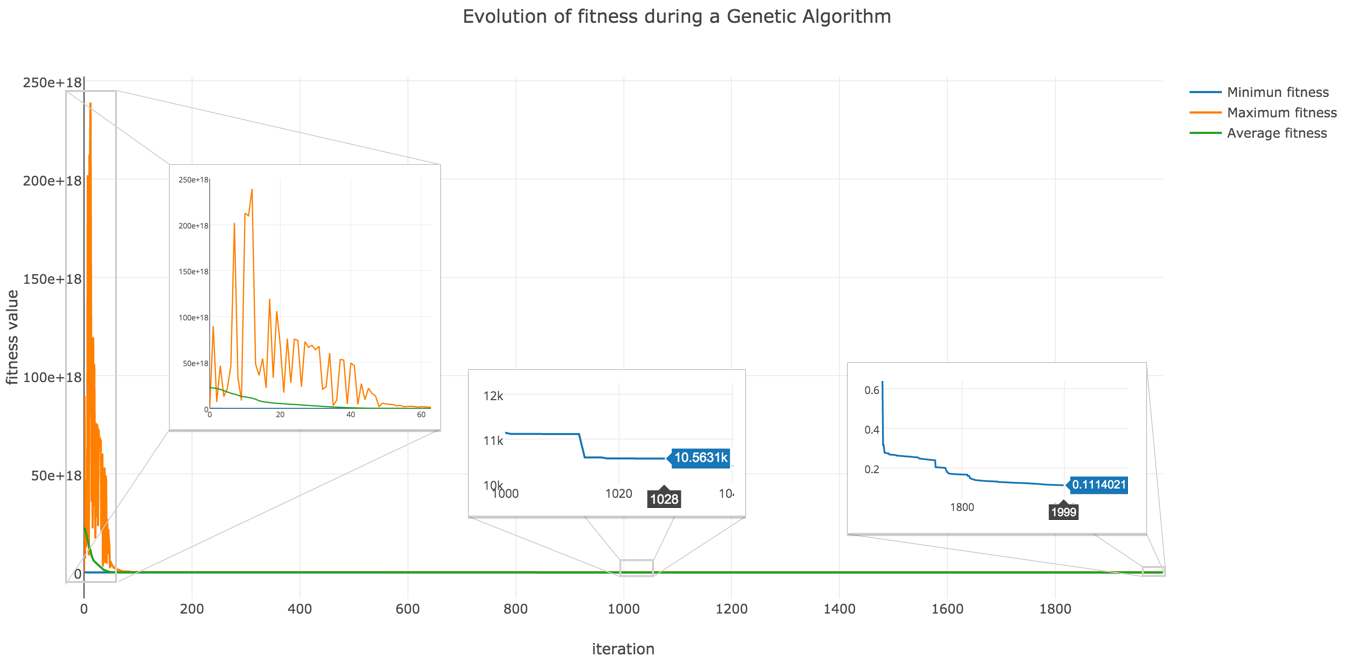
\includegraphics[width=1.0\columnwidth, angle=270]{./plot_fitness_evolution.png}
	\caption{Evolution of fitness during a Genetic Algorithm}
\end{figure}

\section{Formulation of our best solution}

$$f(x) = 0.0 + 5000.0*x + 5.0*x^2 - 62.0*x^3 + 1.0*x^4 - 0.001*x^5$$

\section{Plot of our best solution compared to the target one}

\begin{figure}[H]
	\centering
	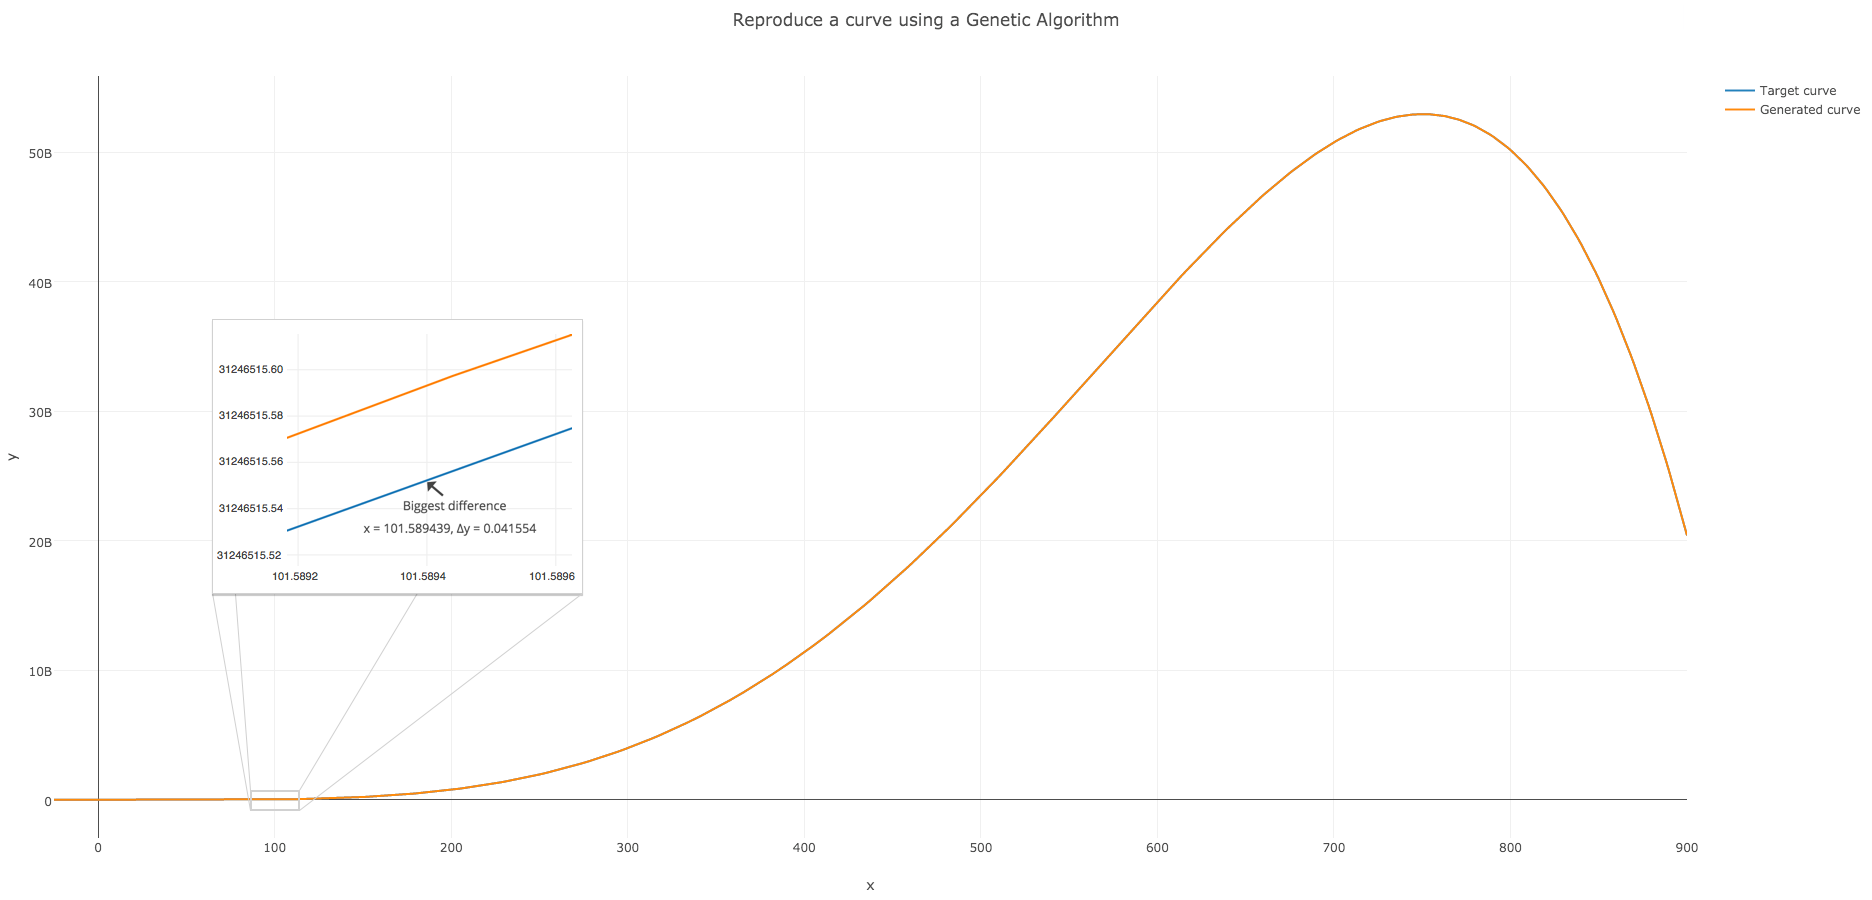
\includegraphics[width=1.0\columnwidth, angle=270]{./plot_solution.png}
	\caption{Reproduce a curve using a Genetic Algorithm}
\end{figure}

\end{document}
